\section{Experiment 1. Baseline performance across penalties}
\label{sec:exp1}
We compare four methods at \(c\in\{0,3,10,30\}\), using ten seeds per method and penalty, for 160 runs in total. Table~\ref{tab:exp1} shows that the relative performance depends on the target. At \(c=0\), each adaptive method discovers B in nine runs, but BO-EI and TuRBO-1 attain precision in all nine, compared with two CMA-ES runs. As the penalty increases, discovery becomes less frequent for the BO variants. At \(c=10\), both attain discovery and precision twice, whereas CMA-ES discovers B seven times but reaches precision only twice. Such observation suggests that while CMA-ES is capable of discovering the optimum basin in multiple instances, it is less able to refine to the global minimum solution; BO and its variants have the opposite problem, being able to refine to a minimum solution but unable to discover the optimum basin.

\begin{table}[!htb]
 \centering
 \caption{Discovery / precision counts after 50 evaluations, out of ten runs per data point.}
 \label{tab:exp1}
 \begin{tabular}{rcccc}
 \toprule
 \(c\) & BO-EI & TuRBO-1 & CMA-ES & Uniform random\\
 \midrule
 0  & 9/9 & 9/9 & 9/2 & 10/1\\
 3  & 5/5 & 5/5 & 9/2 & 10/1\\
 10 & 2/2 & 2/2 & 7/2 & 9/1\\
 30 & 1/1 & 1/0 & 5/0 & 8/1\\
 \bottomrule
 \end{tabular}
\end{table}

Uniform random search has the highest observed discovery count at every penalty, but attains precision only once in each setting. We can derive that for \(T\) independent uniform evaluations,
\begin{equation}
\label{eq:uniform}
 \Pr(D_T)=
 1-\left(1-\frac{\pi\rho_c^2}{64}\right)^T,
 \qquad
 \Pr(P_T)=
 1-\left(1-\frac{\pi(0.1)^2}{64}\right)^T.
\end{equation}
where $D_T$ and $P_T$ denotes the event of already attaining discovery and precision by the $t^{th}$ evaluation, respectively. At \(T=50\), the precision probability is only about \(2.43\%\). Broad coverage can therefore produce frequent discoveries while remaining inefficient for precision. 

\begin{figure}[!htb]
 \centering
 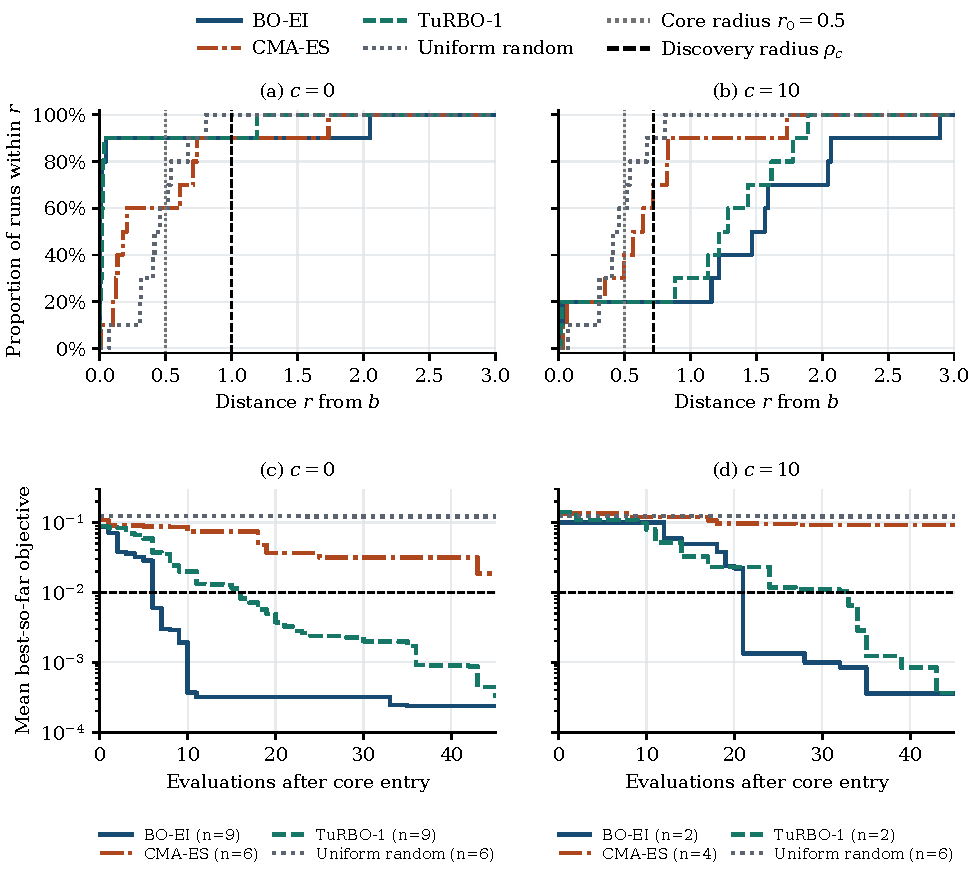
\includegraphics[width=.82\linewidth]{experiment1_c0_c10.pdf}
 \caption{Closest approach to \(b\) (top) and best-so-far values
 after first core entry (bottom), at \(c=0\) and \(c=10\).
 Only core-entering runs appear below. Crosses mark the final
 available evaluations; the dashed horizontal line is the
 precision threshold.}
 \label{fig:experiment1_diagnostics}
\end{figure}

Figure~\ref{fig:experiment1_diagnostics} illustrates such point. At \(c=10\), CMA-ES samples within distance 1 of \(b\) in nine runs, compared with two for BO-EI and three for TuRBO-1. Because this neighbourhood has fixed size, the difference cannot be explained solely by the shrinking discovery threshold as $c$ increases. CMA-ES enters the fixed core in four runs, compared with two for each BO variant, but all three attain precision twice. At \(c=0\), both BO variants attain precision in all nine core-entering runs, compared with two of six for CMA-ES.

These observations suggest a discovery bottleneck for the BO variants and less reliable refinement for default CMA-ES. We next test whether changing global coverage or sampling concentration alters the corresponding outcome. 